\ifx\PREAMBLE\undefined
\documentclass{report}
\usepackage[format = hang, font = bf]{caption}
\usepackage{graphicx}
\usepackage{array}
\usepackage{amsmath}
\usepackage{mathtools}
\usepackage{boxedminipage}
\usepackage{listings}
\usepackage{makecell}%diagonal line in table
\usepackage{float}%allowing forceful figure[H]
\usepackage{xcolor}
\usepackage{amsfonts}%allowing \mathbb{R}
\usepackage{alltt}
\usepackage{algorithmicx}
\usepackage[chapter]{algorithm} 
%chapter option ensures that algorithms are numbered within each chapter rather than in the whole article
\usepackage[noend]{algpseudocode} %If end if, end procdeure, etc is expected to appear, remove the noend option
\usepackage{xspace}
\usepackage{color}
\usepackage{url}
\def\UrlBreaks{\do\A\do\B\do\C\do\D\do\E\do\F\do\G\do\H\do\I\do\J\do\K\do\L\do\M\do\N\do\O\do\P\do\Q\do\R\do\S\do\T\do\U\do\V\do\W\do\X\do\Y\do\Z\do\[\do\\\do\]\do\^\do\_\do\`\do\a\do\b\do\c\do\d\do\e\do\f\do\g\do\h\do\i\do\j\do\k\do\l\do\m\do\n\do\o\do\p\do\q\do\r\do\s\do\t\do\u\do\v\do\w\do\x\do\y\do\z\do\0\do\1\do\2\do\3\do\4\do\5\do\6\do\7\do\8\do\9\do\.\do\@\do\\\do\/\do\!\do\_\do\|\do\;\do\>\do\]\do\)\do\,\do\?\do\'\do+\do\=\do\#\do\-}
\usepackage[breaklinks = true]{hyperref}
\lstset{language = c++, breaklines = true, tabsize = 2, numbers = left, extendedchars = false, basicstyle = {\ttfamily \footnotesize}, keywordstyle=\color{blue!70}, commentstyle=\color{red!70}, frame=shadowbox, rulesepcolor=\color{red!20!green!20!blue!20}, numberstyle={\color[RGB]{0,192,192}}}
\mathchardef\myhyphen="2D
% switch-case environment definitions
\algblock{switch}{endswitch} 
\algblock{case}{endcase}
%\algrenewtext{endswitch}{\textbf{end switch}} %If end switch is expected to appear, uncomment this line.
\algtext*{endswitch} % Make end switch disappear
\algtext*{endcase}
\begin{document}
\fi
\chapter{Code generation}
\section{Stack machines}
A stack machine uses only a stack as storage. When executing an instruction $\mathtt{r = F(a_1,\dots,a_n)}$, it pops n operands from the stack, computes the operation F using the operands, and pushes the result r back on the stack. For example, when computing 7 + 5, the stack will change from s-7-5 to s-12. 

Consider two instructions: push i (push integer i on the stack) and add (add two integers). Then we have the program to computer 7 + 5:
\begin{center}
push 7\\push 5\\add
\end{center}
An important property of stack machines is that location of the operands/result is not explicitly stated because they are always at the top of the stack. This is different from register machine in which the locations have to be specified. We have \texttt{add} instead of \texttt{add} $\mathtt{r_1, r_2, r_3}$, which produces more compact programs. This is one of the reasons why JAVA bytecodes uses stack evaluation.

Stack machine produces compact programs, but register machine executes faster. There is an intermediate point between the two kinds of machines called an \textbf{n-register stack machine}. As the name reveals, the top n positions of the pure stack machine's stack are held in registers. It turns out that even one single register can provide considerable performance improvement, which is the case of \textbf{1-register stack machine}. The register is called the \textbf{accumulator}. 

In a pure stack machine, an add does 3 memory operations: two reads and one write. But in a 1-register stack machine, what add does is acc$\leftarrow$acc + top\_of\_stack. In general, consider an arbitrary expression $\mathtt{op(e_1,\dots,e_n)}$. For each subexpression $e_i(1\leq i\leq n-1)$, we will compute $e_i$, store the result in acc and then push the result on the stack. For $e_n$, we will have its result remain in acc. Then we will pop n-1 values from the stack to compute op, and store the result in acc. If we follow this procedure, obviously after evaluating an expression e, acc holds the value of e, and the stack is unchanged. In other words, \textbf{expression evaluation preserves the stack.}

Consider the calculation of 3 + (7 + 5). We will have the following process:
\begin{table}[ht]
\centering
\begin{tabular}{lcc}
Code & Acc & Stack\\
acc$\leftarrow$3 & 3 & $<$init$>$\\
push acc & 3 & 3,$<$init$>$\\
acc$\leftarrow$7 & 7 & 3,$<$init$>$\\
push acc & 7 & 7,3,$<$init$>$\\
acc$\leftarrow$5 & 5 & 7,3,$<$init$>$\\
acc$\leftarrow$acc + top\_of\_stack & 12 & 7,3,$<$init$>$\\
pop & 12 & 3,$<$init$>$\\
acc$\leftarrow$acc + top\_of\_stack & 15 & 3,$<$init$>$\\
pop & 15 & $<$init$>$
\end{tabular}
\end{table}
\section{Basic MIPS instructions}
In our discussion of code generation, we will focus on generating code for a stack machine with accumulator. The resulting code should be able to run on an MIPS processor (or simulator). Thus we have to simulate stack machine instructions using MIPS instructions and registers.

We choose to keep the accumulator in MIPS register \$a0. The stack is kept in memory and grows towards lower addresses, which is a standard convention in MIPS. The address of the next location on the stack is kept in MIPS register \$sp (which stands for stack pointer), and the top of the stack is at address \$sp + 4.

MIPS is an old structure with a relatively simple instruction set (prototypical reduced instruction set computer, or RISC). Most MIPS operations use registers for operands and results. Load and store instructions are used to move values to and from memory. There are 32 general purpose registers (32 bits each) in MIPS, and we will use only \$a0, \$sp and \$t1 (temp register used for operations that take two arguments). 

Here are the first set of MIPS instructions that we introduce.
\begin{description}
\item[lw reg1 offset(reg2)]: Load 32-bit word from address \texttt{reg2 + offset} into \texttt{reg1}. 
\item[sw reg1 offset(reg2)]: Store 32-bit word in \texttt{reg1} at address \texttt{reg2 + offset}.
\item[add reg1 reg2 reg3]: \texttt{reg1 $\leftarrow$ reg2 + reg3}
\item[addiu reg1 reg2 imm]: \texttt{reg1 $\leftarrow$ reg2 + imm. u} means that overflow is not checked.
\item[li reg imm]: \texttt{reg $\leftarrow$ imm}.
\item[move reg1 reg2] reg1 $\leftarrow$ reg2.
\end{description}
The stack machine code for 7 + 5 is: 
\begin{table}[h]
\tt 
\centering
\begin{tabular}{ll}
acc $\leftarrow$ 7  & li \$a0 7 \\
push acc 			& sw \$a0 0(\$sp)\\
					& addiu \$sp \$sp -4 \\
acc $\leftarrow$ 5  & li \$a0 5 \\
acc $\leftarrow$ acc + top\_of\_stack & lw \$t1 4(\$sp) \\
									  & add \$a0 \$a0 \$t1 \\
pop & addiu \$sp \$sp 4
\end{tabular}
\end{table}
\section{Code generation for a simple language}
In this section we will take a look at code generation for higher level languages rather than a simple stack machine in the previous section.

Consider a language for integer operations. Its grammar depicts a list of function definitions:
\begin{align*}
&\mathsf{P\rightarrow D;\:P\:|\:D}\\
&\mathsf{D\rightarrow def\:id(ARGS)\:=\:E}\\
&\mathsf{ARGS\rightarrow\:id,\:ARGS\:|\:id}\\
&\mathsf{E\rightarrow\:int\:|\:id\:|\:if\:E_1\:=\:E_2\:then\:E_3\:else\:E_4\:|\:E_1\:+\:E_2\:|\:E_1\:-\:E_2\:|\:id(E_1,\dots,E_n)}
\end{align*}
The first function definition \texttt{f} is the entry point, i.e. the \texttt{main} routine. This language is enough to write a program that computes the Fibonacci numbers:
\begin{equation}\label{fibonacci}\begin{split}
\texttt{def fib(x) = }&\texttt{if x = 1 then 0 else}\\
&\texttt{if x = 2 then 1 else}\\
&\texttt{fib(x - 1) + fib(x - 2)}
\end{split}\end{equation}
For each expression \texttt{e}, we want to generate MIPS code that \textbf{computers the value of \texttt{e} in \$a0} and \textbf{preserves \$sp and the content of the stack}. We will define a function \texttt{cgen(e)} whose return value if the code generated for \texttt{e}.

\subsection{Constants}
For constants, we need to simply load it into the accumulator:
\begin{center}
\texttt{\color{red}cgen(i)}\texttt{ = li \$a0 i}
\end{center}
\subsection{Addition}
For addition:
\begin{align*}
\texttt{\color{red}cgen(e1 }&\texttt{\color{red}+ e2) }=\\
&\texttt{\color{red}cgen(e1)}\\
&\texttt{sw \$a0 0(\$sp)}\\
&\texttt{addiu \$sp \$sp -4}\\
&\texttt{\color{red} cgen(e2)}\\
&\texttt{lw \$t1 4(\$sp)}\\
&\texttt{add \$a0 \$t1 \$a0}\\
&\texttt{addiu \$sp \$sp 4}
\end{align*}
Here we use different colors to emphasize the fact that MIPS code is \textbf{generated} at compile time and \textbf{executed} at run time. Code in red color is what happens at compile time: the generation, while code in black is what happens at run time: the execution. More precisely, we should write \texttt{sw \$a0 0(\$sp)} as something like \texttt{{\color{red}print} sw \$a0 0(\$sp)}, which indicates that the MIPS code is generated at compile time and saved somewhere, maybe in an intermediate file, and does not get executed until run time.

It seems that the piece of code above could be optimized: why don't we save the value of e1 directly in \$t1, rather than saving it in the memory and then retrieve it into \$t1? The code will look like:
\begin{align*}
\texttt{\color{red}cgen(e1 }&\texttt{\color{red}+ e2) }=\\
&\texttt{\color{red}cgen(e1)}\\
&\texttt{move \$t1 \$a0}\\
&\texttt{\color{red} cgen(e2)}\\
&\texttt{add \$a0 \$t1 \$a0}
\end{align*}
Unfortunately, this neat piece of code is wrong. We can convince ourselves by simply considering the code generated for 1 + (2 + 3). In short, the value of \$t1 will be modified during \texttt{cgen(e2)}, and is no longer the value of e1 when the execution comes to \texttt{add \$a0 \$t1 \$a0}.

The simple example of code generation for addition demonstrates a few universal properties of code generation. The code generated for \texttt{e1 + e2} is a template with ``holes'' for code generated to evaluate e1 and e2. Stack machine code generation is actually recursive. The code generation process can be written as a recursive descent of the AST, at least for expressions.

\subsection{Subtraction}
By introducing another MIPS instruction sub:
\begin{description}
\item[sub reg1 reg2 reg3] reg1$\leftarrow$reg2 - reg3
\end{description}
we can generate the code for \texttt{e1 - e2}:
\begin{align*}
\texttt{\color{red}cgen(e1 }&\texttt{\color{red}- e2) }=\\
&\texttt{\color{red}cgen(e1)}\\
&\texttt{sw \$a0 0(\$sp)}\\
&\texttt{addiu \$sp \$sp -4}\\
&\texttt{\color{red}cgen(e2)}\\
&\texttt{lw \$t1 4(\$sp)}\\
&\texttt{sub \$a0 \$t1 \$a0}\\
&\texttt{addiu \$sp \$sp 4}
\end{align*}

\subsection{If-then-else}
In order to generate code for \texttt{if-then-else} expressions, we need to introduce a couple of new instructions:
\begin{description}
\item[beq reg1 reg2 label] branch to label if reg1 = reg2
\item[b label] Unconditional jump to label
\end{description}
\begin{align*}
\texttt{\color{red}cgen(if e1 = e2 }&\texttt{\color{red}then e3 else e4) }=\\
&\texttt{\color{red}cgen(e1)}\\
&\texttt{sw \$a0 0(\$sp)}\\
&\texttt{addiu \$sp \$sp -4}\\
&\texttt{\color{red}cgen(e2)}\\
&\texttt{lw \$t1 4(\$sp)}\\
&\texttt{addiu \$sp \$sp 4}\\
&\texttt{beq \$t1 \$a0 true\_branch}\\
&\texttt{false\_branch:}\\
&\texttt{\quad\color{red}cgen(e4)}\\
&\texttt{\quad b end\_if}\\
&\texttt{true\_branch:}\\
&\texttt{\quad\color{red}cgen(e3)}\\
&\texttt{end\_if:}
\end{align*}

\subsection{Function calls \& definitions, variable references}
Code for function calls and function definitions depends on the layout of the activation record, thus they need to be designed together. For this simple language, a very simple AR is sufficient. 
\begin{itemize}
\item Since the result is always in the accumulator, there is no need to store the result in AR. 
\item The AR should hold the actual parameters, thus for $f(x_1,\dots,x_n)$, we need to push $x_n,\dots,x_1$ on the stack. These are the only variables in this language. 
\item The stack discipline guarantees that \$sp is preserved after a function call. Thus there is no need for a control link: the previous activation can be found directly; and we do not need to look at another activation during the function call because there is no non-local variable. 
\item We need the return address.
\item A pointer to the \textbf{current} activation is useful. It lives in register \$fp (frame pointer).
\end{itemize}
To summarize, for this simple language, an AR will contain the caller's frame pointer, the actual parameters and the return address. The caller's frame pointer should be contained because \$fp will be probably overwritten during the execution of the function (by other functions called during the execution). Consider a call to $f(x,y)$. Before its body gets executed, its AR looks like Figure \ref{aroff}.
\begin{figure}[ht]
\centering
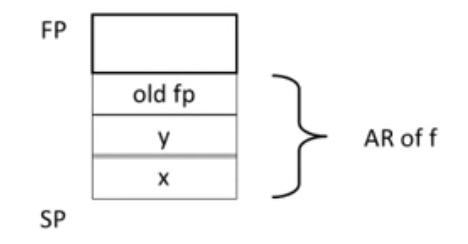
\includegraphics[width=0.5\textwidth]{aroff.jpg}
\caption{AR of f(x,y)}\label{aroff}
\end{figure}
The \textbf{calling sequence} is the instructions (of both the caller and the callee) to set up a function invocation. Here we introduce a new instruction
\begin{description}
\item[jal label] Jump to label, and save the address of the next instruction in \$ra (meaning return address). \textbf{jal} means jump and link.
\end{description}
Now we can actually generate the code for function call expressions. 
\begin{align*}
\texttt{\color{red}cgen}&\texttt{\color{red}(f(e1,e2,...,en)) }=\\
&\texttt{sw \$fp 0(\$sp)}\\
&\texttt{addiu \$sp \$sp -4}\\
&\texttt{\color{red}cgen(en)}\\
&\texttt{sw \$a0 0(\$sp)}\\
&\texttt{addiu \$sp \$sp -4}\\
&\dots\\
&\texttt{\color{red}cgen(e1)}\\
&\texttt{sw \$a0 0(\$sp)}\\
&\texttt{addiu \$sp \$sp -4}\\
&\texttt{jal f\_entry}
\end{align*}
For \texttt{f(e1,e2,...,en)}, we first save the frame pointer of the caller, then save the arguments one by one (from \texttt{en} to \texttt{e1}). Up to now we've completed the calling sequence on the caller side. Next we can use \texttt{jal} to jump to the entry point of function \texttt{f}. The return address is now in \$ra. The AR so far is \texttt{4*n+4} bytes long.  

We introduce another instruction
\begin{description}
\item[jr reg]Jump to the address in register reg.
\end{description}
Now we can discuss the callee side of the calling sequence. 
\begin{align*}
\texttt{\color{red}cgen}&\texttt{\color{red}(def f(x1,x2,...,xn) = e) }=\\
&\texttt{f\_entry:}\\
&\quad\texttt{move \$fp \$sp}\\
&\quad\texttt{sw \$ra 0(\$sp)}\\
&\quad\texttt{addiu \$sp \$sp -4}\\
&\quad\texttt{\color{red}cgen(e)}\\
&\quad\texttt{lw \$ra 4(\$sp)}\\
&\quad\texttt{addiu \$sp \$sp 4n + 8}\\
&\quad\texttt{lw \$fp 0(\$sp)}\\
&\quad\texttt{jr \$ra}\\
\end{align*}
First we set up the frame pointer by saving the current stack pointer into \$fp. Then the return address is saved in memory. Now we can generate code for the function body. The stack pointer will be reserved, thus we can load the return address back into \$ra. Next we can pop the return address, all arguments and the old fp out of the stack (totally 4*n+8 bytes). We restore the value of the old fp, and finally jump back to the return address. 

Variables in this language are just the function arguments. They are all pushed into the AR by the caller. But since the stack grows when intermediate results are saved, the variables are not at fixed offsets from \$sp. That's when \$fp should be used. The offset of \texttt{xi} from \$fp is 4*i. Thus we can generate the code for variable reference. 
\begin{equation*}
\texttt{\color{red}cgen(xi)}\texttt{ = lw \$a0 4*i(\$fp)}
\end{equation*}
\subsection{Summary}
To summarize, the AR must be designed together with the code generator. Code generation can be completed by a recursive traversal of the AST. Such an approach using a stack machine is a wise choice to implement the COOL code generator. 

Production compilers are for sure different from the example here. They emphasize keeping values in registers, especially the current stack frame, for the code to run faster. Also, intermediate results are laid out in the AR rather than pushed and popped from the stack. 

As an example, let's generate the code for the following program:
\begin{lstlisting}
def sumto(x) = if x = 0 then 0 else x + sumto(x - 1)
\end{lstlisting}
\begin{align*}
&\texttt{sumto\_entry:}&&\\
&\quad\texttt{move \$fp \$sp}&//&\text{set up frame pointer}\\
&\quad\texttt{sw \$ra \$sp}&//&\text{return address}\\
&\quad\texttt{addiu \$sp \$sp -4}&&\\
&\quad\texttt{lw \$a0 4(\$fp)}&//&\text{start generation for if-then-else. load x from AR.}\\
&\quad\texttt{sw \$a0 0(\$sp)}&//&\text{save value of x (1st arg of comparison)}\\
&\quad\texttt{addiu \$sp \$sp -4}&&\\
&\quad\texttt{li \$a0 0}&//&\text{immediately load 0}\\
&\quad\texttt{lw \$t1 4(\$sp)}&//&\text{load x (1st arg of comparison) into \$t1}\\
&\quad\texttt{addiu \$sp \$sp 4}&//&\text{pop x}\\
&\quad\texttt{beq \$t1 \$a0 true1}&//&\text{compare and branch}\\
&\texttt{false1:}&&\\
&\quad\texttt{lw \$a0 4(\$fp)}&//&\text{load x from AR}\\
&\quad\texttt{sw \$a0 0(\$sp)}&//&\text{save value of x (1st arg of addition)}\\
&\quad\texttt{addiu \$sp \$sp -4}&&\\
&\quad\texttt{sw \$fp 0(\$sp)}&//&\text{save frame pointer of caller}\\
&\quad\texttt{addiu \$sp \$sp -4}&&\\
&\quad\texttt{lw \$a0 4(\$fp)}&//&\text{load x from AR}\\
&\quad\texttt{sw \$a0 0(\$sp)}&//&\text{save value of x (1st arg of subtraction)}\\
&\quad\texttt{addiu \$sp \$sp -4}&&\\
&\quad\texttt{li \$a0 1}&//&\text{immediately load 1}\\
&\quad\texttt{lw \$t1 4(\$sp)}&//&\text{load x (1st arg of subtraction into \$t1)}\\
&\quad\texttt{sub \$a0 \$t1 \$a0}&//&\text{subtraction}\\
&\quad\texttt{addiu \$sp \$sp 4}&//&\text{pop x}\\
&\quad\texttt{sw \$a0 0(\$sp)}&//&\text{save value of x-1 (arg of sumto(x-1))}\\
&\quad\texttt{addiu \$sp \$sp -4}\\
&\quad\texttt{jal sumto\_entry}&//&\text{jump and link}\\
&\quad\texttt{lw \$t1 4(\$sp)}&//&\text{load x (1st arf of addition) into \$t1}\\
&\quad\texttt{add \$a0 \$t1 \$a0}&//&\text{addition (x+sumto(x-1))}\\
&\quad\texttt{addiu \$sp \$sp 4}&//&\text{pop x. up to now finished x+sumto(x-1)}\\
&\quad\texttt{b end\_if1}&&\\
&\texttt{true1:}&&\\
&\quad\texttt{li \$a0 0}&//&\text{immediately load 0}\\
&\texttt{end\_if1}&//&\text{up to now finished if-then-else}\\
&\quad\texttt{lw \$ra 4(\$sp)}&//&\text{load return address}\\
&\quad\texttt{addiu \$sp \$sp 12}&//&\text{pop ra, argument(x) and old fp}\\
&\quad\texttt{lw \$fp 0(\$sp)}&//&\text{restore old fp}\\
&\quad\texttt{jr \$ra}&&\\
\end{align*}
\section{Temporaries}
One of the advantages of production compilers over the simple one we introduced is that temporaries are kept in the AR. In order to generate more efficient code, the code generator must assign a fixed location in the AR for each temporary. If we use NT(e) to represent the number of temporaries to evaluate expression e. We will have 
\begin{align*}
NT(e_1 + e_2)&=\max(NT(e_1), 1 + NT(e_2))\\
NT(e_1 - e_2)&=\max(NT(e_1), 1 + NT(e_2))\\
NT(\text{if }e_1 = e_2\text{ then }e_3\text{ else }e_4)&=\max(NT(e_1), 1 + NT(e_2), NT(e_3), NT(e_4))\\
NT(id(e_1,\dots,e_n))&=\max(NT(e_1),\dots,NT(e_n))\\
NT(int)&=0\\
NT(id)&=0\\
\end{align*}
The rule for $id(e_1,\dots,e_n)$ is correct because the temps to store $e_1,\dots,e_{i-1}$ are stored in the new AR, not the current AR. 

Consider the Fibonacci function \eqref{fibonacci}. With the rules above applied, 2 temps are enough to evaluate it.

For a function definition \texttt{def f(x1,...,xn) = e}, the AR has \texttt{2 + n + NT(e)} elements: return address, frame pointer, n arguments and NT(e) locations for intermediate results. The layout of the AR is shown in Figure 
\ref{arlayout}.
\begin{figure}[ht]
\centering
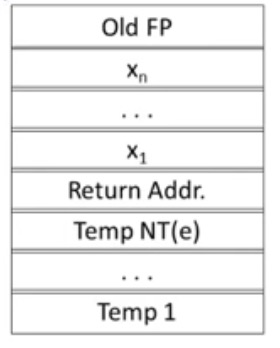
\includegraphics[width = 0.4\textwidth]{arlayout.jpg}
\caption{Layout of AR}\label{arlayout}
\end{figure}

Now that we have knowledge of how many temps are needed to evaluate a function and where they are going to be stored in the AR, what's left is to keep track of how many temps are in use at each point in the program. To achieve this, we will add a new argument to code generation: \textbf{the position of the next available temp}. The temp area will be used like a small, fixed-size stack. 

Here is the old code generation for \texttt{e1 + e2}:
\begin{align*}
\texttt{\color{red}cgen(e1 }&\texttt{\color{red}+ e2) }=\\
&\texttt{\color{red}cgen(e1)}\\
&\texttt{sw \$a0 0(\$sp)}\\
&\texttt{addiu \$sp \$sp -4}\\
&\texttt{\color{red} cgen(e2)}\\
&\texttt{lw \$t1 4(\$sp)}\\
&\texttt{add \$a0 \$t1 \$a0}\\
&\texttt{addiu \$sp \$sp 4}
\end{align*}
Under the new scheme, code generation will take a new argument:
\begin{align*}
\texttt{\color{red}cgen(e1 }&\texttt{\color{red}+ e2, nt) }=\\
&\texttt{\color{red}cgen(e1, nt)}\\
&\texttt{sw \$a0 nt(\$fp)}\\
&\texttt{\color{red} cgen(e2, nt + 4)}\\
&\texttt{lw \$t1 nt(\$fp)}\\
&\texttt{add \$a0 \$t1 \$a0}\\
\end{align*}
\section{Object layout}
In this section we will focus on code generation for a more advanced feature: objects.

In OO programming, if B is a subclass of A, the an object of class B can be used whenever an object of class A is used, which means that code generated for class A has to work without any modification for class B. To give a complete description of the code generation for objects, two questions need to be answered:
\begin{itemize}
\item How are objects represented in memory?
\item How is dynamic dispatch implemented?
\end{itemize}
We will use the following COOL code to illustrate the code generation for objects.
\begin{lstlisting}
class A {
	a:Int <- 0;
	d:Int <- 1;
	f():Int { a <- a + d };
};
class B inherits A {
	b:Int <- 2;
	f():Int { a };
	g():Int { a <- a - b };
};
class C inherits A {
	c:Int <- 3;
	h():Int { a <- a * c };
}
\end{lstlisting}

\texttt{A} is the base class while \texttt{B} and \texttt{C} inherits from it. Note that attributes \texttt{a} and \texttt{d} are inherited by \texttt{B} and \texttt{C}, and that \texttt{a} is used in all methods of the 3 classes. For these methods to work correctly, attribute \texttt{a} must be in the same ``place'' in each object. To ensure this, 2 conditions have to be satisfied: 
\begin{itemize}
\item Objects are laid out in contiguous memory.
\item Each attribute is stored at a fixed offset in the object. 
\end{itemize}
Let's take a look at the layout of an object in COOL, as shown in Figure \ref{coolobjlayout}. 
\begin{figure}[ht]
\centering
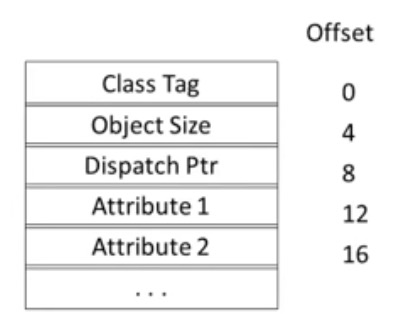
\includegraphics[width=0.5\textwidth]{coolobjlayout.jpg}
\caption{Layout of COOL object}\label{coolobjlayout}
\end{figure}
The first 3 words are always header information. \textbf{Class tag} is an integer that identifies the class of the object. \textbf{Object size} is an integer that specifies the size of the object in words. \textbf{Dispatch pointer} is a pointer to a table of methods, which will be explained in detail later. They are followed by attributes of the class in subsequent slots. All these are laid out in contiguous memory. 

Given the layout of class A, the layout of its subclass B can be defined by extending the layout of A with additional slots for the additional attributes of B. Thus the layout of A is left unchanged. 

In our example, the layout of the 3 classes are shown in Table \ref{layoutabc}.
\begin{table}[ht]
\centering
\caption{Layout of classes \texttt{A,B,C}}\label{layoutabc}
\begin{tabular}{|c|c|c|c|c|c|c|}\hline
\diaghead(3,-1){\hskip2cm}%
{class}{offset} & 0 & 4 & 8 & 12 & 16 & 20\\\hline
A & Atag & 5 & * & a & d & \\\hline
B & Btag & 6 & * & a & d & b \\\hline
C & Ctag & 6 & * & a & d & c \\\hline
\end{tabular}\end{table}
In general, if B is a subclass of A, then an A object is ``nested'' inside an B object.

Every class has a fixed set of methods, including inherited methods. A \textbf{dispatch table} indexes these methods. It is an array of method entry points. A method \texttt{f} lives at a fixed offset in the dispatch table for a class and all of its subclasses. The dispatch tables of classes \texttt{A,B,C} are shown in Table \ref{dispatchtables}.
\begin{table}[ht]
\centering
\caption{Dispatch tables of classes \texttt{A,B,C}}\label{dispatchtables}
\begin{tabular}{|c|c|c|}\hline
\diaghead(3,-1){\hskip2cm}%
{class}{offset} & 0 & 4 \\\hline
A & fA & \\\hline
B & fB & g \\\hline
C & fA & h \\\hline
\end{tabular}\end{table}
The dispatch pointer in an object of class X points to the dispatch table of class X. The reason for which we use a pointer to the dispatch table rather than putting all the methods in each object directly is that each object can have its own copy of the attributes, but the methods are always the same. 

Every method f of class X is assigned an offset $O_f$ in the dispatch table at compile time. To implement a dynamic dispatch \texttt{e.f()}, we will evaluate \texttt{e} to get an object \texttt{x}, and then call $D[O_f]$, in which $D$ is the dispatch table for \texttt{x}. In the call, \texttt{self} is bound to \texttt{x}. 
\section{Semantics}
\ifx\PREAMBLE\undefined
\end{document}
\fi